\chapter{System Overview} \label{overview}

Figure~\ref{fig:overview} shows the main components of External Debug Support.
Blocks shown in dotted lines are optional. 

\begin{figure}
   \centering
   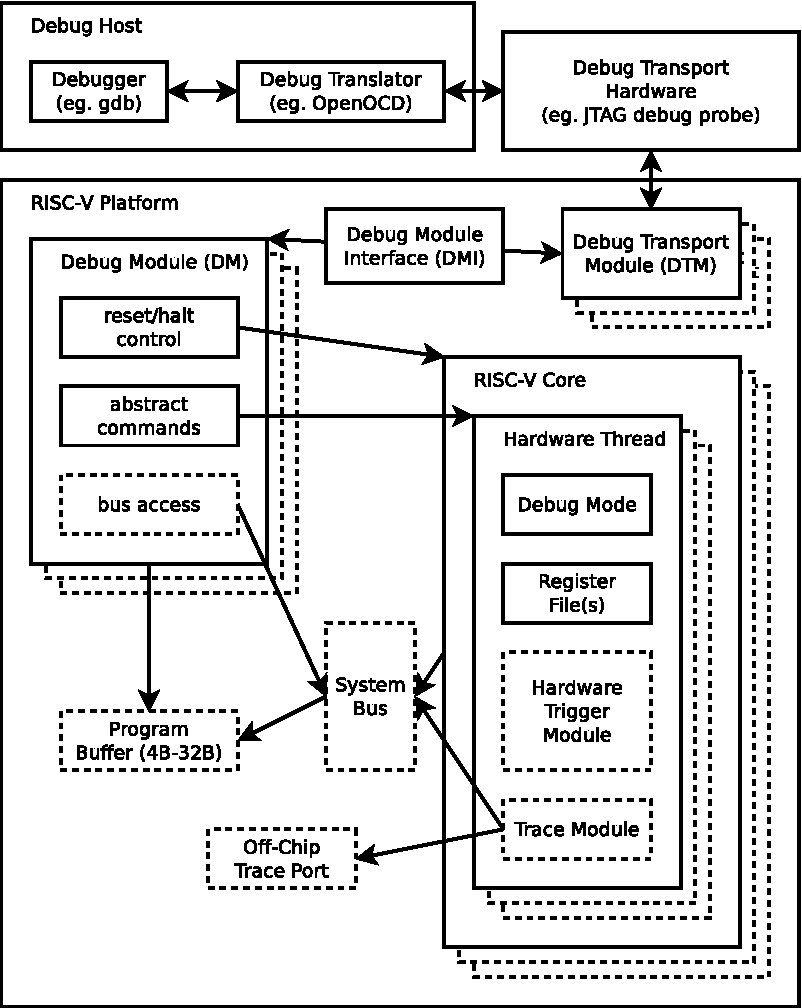
\includegraphics[width=\textwidth]{fig/overview-eps-converted-to.pdf}
   \caption{RISC-V Debug System Overview}
   \label{fig:overview}
\end{figure}

The user interacts with the Debug Host (eg. laptop), which is running a
debugger (eg. gdb).  The debugger communicates with a Debug Translator (eg.
OpenOCD, which may include a hardware driver) to communicate with Debug
Transport Hardware (eg.  Olimex USB-JTAG adapter).
The Debug Transport Hardware connects the Debug Host to the Platform's Debug
Transport Module (DTM).  The DTM provides access to the Debug Module (DM) using
the Debug Module Interface (DMI).

The DM allows the debugger to halt any hart in the platform. Abstract commands
provide access to GPRs.
The optional Program Buffer allows the debugger to execute arbitrary code on the hart,
which allows access to additional hart state. Alternatively, additional
abstract commands can provide access to additional hart state.

Each RISC-V hart may implement a Trigger Module. When trigger conditions
are met, harts will halt and inform the debug module that they have
halted.

An optional system bus access block allows memory accesses without using a
RISC-V hart to perform the access.

Optional serial port blocks allow the Debug Transport to be re-used as a
generic communication interface.
